\documentclass[12,french]{report}
\usepackage{geometry}
\geometry{vmargin=3cm, hmargin=3cm}
\usepackage[T1]{fontenc}
\usepackage[utf8]{inputenc}
\usepackage[french]{babel}
\usepackage{graphicx}
\usepackage{amsmath}
\usepackage{amssymb}
\usepackage{sectsty}
\usepackage{authblk}
\usepackage{algpseudocode}
\usepackage{algorithm}
\usepackage{xspace}
\usepackage{mathtools}
\usepackage{mathrsfs}
\usepackage{enumitem}
\usepackage{titlesec}
\usepackage{hyperref}
\usepackage{xcolor}
\usepackage[justification=centering]{caption}
\usepackage{float}
\usepackage{tabto}

\usepackage{listings}
\usepackage{cleveref}

\renewcommand{\lstlistingname}{Code}
%\renewcommand{\figurename}{Fig.}

\lstdefinestyle{chstyle}{%
backgroundcolor=\color{gray!12},
basicstyle=\ttfamily\small,
showstringspaces=false,
numbers=left}

%\AddThinSpaceBeforeFootnotes
%\FrenchFootnotes

\titleformat{\chapter}[hang]{\bf\Huge}{\thechapter.}{2pc}{}
\titlespacing*{\chapter}{10pt}{0pt}{40pt}[0pt]
\newcommand{\HRule}{\rule{\linewidth}{0.5mm}}

\providecommand{\keywords}[1]{\textbf{\textit{Keywords:}} #1}
\bibliographystyle{apalike}

\usepackage{hyperref}

\begin{document}
\hypersetup{pdfborder=0 0 0}

\begin{titlepage}

\begin{center}
	\vspace*{\stretch{1}}
	\textsc{{\LARGE Institut national des sciences appliquées de Rouen} \\ 			\vspace{6mm} {\Large INSA de Rouen}} \\
	\vspace{5mm}
	
\includegraphics[width=0.4\textwidth]{./Images/insa}\\[1.0 cm]

	\textsc{\Large Projet MSRO GM3 - Vague 2 - Sujet 3}\\[0.6cm]

	% Title
	\HRule \\[0.1cm]
	{ \Huge \bfseries Traitement du signal \\ Etude de deux filtres linéaires}\\[0.2cm]
	\HRule \\[0.95cm]

	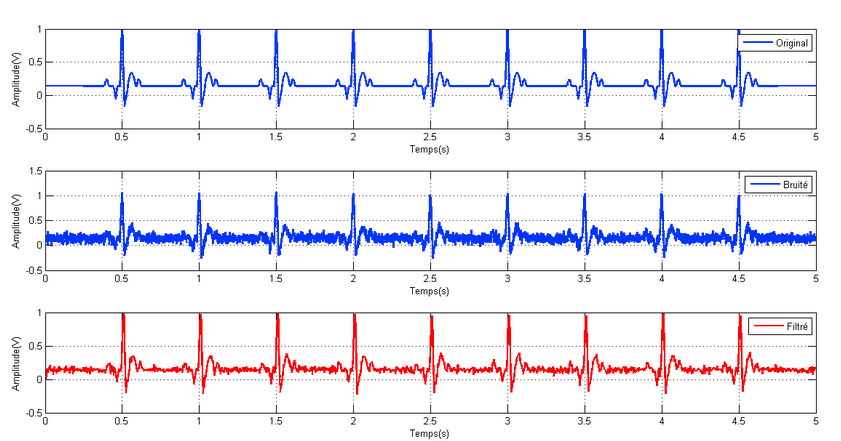
\includegraphics[width=0.8\textwidth]{./Images/Page_de_garde}\\[0.9 cm]

	% Author and supervisor
	\begin{minipage}{0.4\textwidth}
		\begin{flushleft} \large
			\emph{Auteurs:}\\
			Thibaut \textsc{André-Gallis} \\
			{\small\href{mailto:thibaut.andregallis@insa-rouen.fr}{thibaut.andregallis@insa-rouen.fr}} \\
			Kévin \textsc{Gatel} \\
			{\small\href{mailto:kevin.gatel@insa-rouen.fr}{kevin.gatel@insa-				rouen.fr}}
		\end{flushleft}
	\end{minipage}
	\begin{minipage}{0.4\textwidth}
		\begin{flushright} \large
			\emph{Enseignant:} \\
			Natalie \textsc{Fortier} \\
			{\small\href{mailto:natalie.fortier@insa-rouen.fr}								{natalie.fortier@insa-rouen.fr}}
		\end{flushright}
	\end{minipage}
	\vspace*{\stretch{1}}

	\vfill
	{\large 11 Avril 2021}
\end{center}
\end{titlepage}

\tableofcontents

%\listoffigures

\renewcommand{\chaptername}{}
\chapter*{Introduction du problème}

Soit deux filtres $h_k$ et $g_k$ tels que :\\

$$ H(z) = \frac{0.3-0.2z^{-1}+0.4z^{-2}}{1+0.9z^{-1}+0.8z^{-2}} $$
$$ G(z) = \frac{0.2-0.5z^{-1}+0.3z^{-2}}{1+0.7z^{-1}+0.85z^{-2}} $$ \\

Dans un premier temps, on cherche à savoir si ces deux filtres sont réalisables physiquement.\\

On s’intéressera ensuite à la mise en cascade de ces deux filtres pour déterminer s'il agit par équivalence d'un unique filtre. On initialisera ensuite un signal d'entrée pour déterminer la sortie du filtre.\\

Enfin nous étudierons leur mise en parallèle avec les mêmes objectifs que pour la mise en cascade.


\chapter{Filtres réalisables ?}

\section{Pôles}

\subsection{$H(z)$}

\vspace{0.25cm}

On a $$ H(z) = \frac{0.3-0.2z^{-1}+0.4z^{-2}}{1+0.9z^{-1}+0.8z^{-2}} = \frac{0.3z^2-0.2z+0.4}{z^2+0.9z+0.8} $$

Dénominateur : 
$$ D_h= z^2+0.9z+0.8 $$

D'où : $$ \begin{array}{ccl}
\Delta & = & 0.9^2-4*1*0.8 \\
	   & = & -2.39 \\
\end{array} $$

On obtient :
$$\left.\begin{aligned}
	&z_{1Dh} = \frac{-0.9+i\sqrt{2,39}}{2} \\
	&\quad\quad = -0.45 + i\frac{\sqrt{2,39}}{2} \\
\end{aligned}\quad\right|
\quad\left.\begin{aligned}
	&z_{2Dh} = \frac{-0.9-i\sqrt{2,39}}{2}\\
	&\quad\quad = -0.45 - i\frac{\sqrt{2,39}}{2} \\
\end{aligned}\right.$$

Ainsi :
$$ |z_{1Dh}|=|z_{2Dh}|=\sqrt{(-0.45)^2+\left(\frac{\sqrt{2,39}}{2}\right)^2} \simeq 0.89 < 1 $$\\

$H(z)$ a tous ses pôles à l'intérieur du cercle unité \textbf{donc le filtre $h_k$ est réalisable physiquement}.\\

\subsection{$G(z)$}

\vspace{0.25cm}

On a $$ G(z) = \frac{0.2-0.5z^{-1}+0.3z^{-2}}{1+0.7z^{-1}+0.85z^{-2}} = \frac{0.2z^2-0.5z+0.3}{z^2+0.7z+0.85} $$

Dénominateur : $$ D_g= z^2+0.7z+0.85 $$

D'où : $$ \begin{array}{ccl}
\Delta & = & 0.7^2-4*1*0.85 \\
	   & = & -2.91 \\
\end{array} $$

On obtient :
$$\left.\begin{aligned}
	&z_{1Dg} = \frac{-0.7+i\sqrt{2,91}}{2} \\
	&\quad\quad = -0.35 + i\frac{\sqrt{2,91}}{2} \\
\end{aligned}\quad\right|
\quad\left.\begin{aligned}
	&z_{2Dg} = \frac{-0.7-i\sqrt{2,91}}{2}\\
	&\quad\quad =-0.35 - i\frac{\sqrt{2,91}}{2} \\
\end{aligned}\right.$$

Ainsi :
$$ |z_{1Dg}|=|z_{2Dg}|=\sqrt{(-0.35)^2+\left(\frac{\sqrt{2,91}}{2}\right)^2} \simeq 0.92 < 1 $$


$G(z)$ a tous ses pôles à l'intérieur du cercle unité \textbf{donc le filtre $g_k$ est réalisable physiquement}.

\section{Zéros}

\subsection{$H(z)$}

\vspace{0.25cm}

On a $$ H(z) = \frac{0.3z^2-0.2z+0.4}{(z-z_{1Dh})(z-z_{2Dh})} $$

Numérateur : $$ N_h= 0.3z^2-0.2z+0.4 $$

D'où : $$ \begin{array}{ccl}
\Delta & = & (-0.2)^2-4*0.3*0.4 \\
	   & = & -0,44 \\
\end{array} $$

On obtient :
$$\left.\begin{aligned}
	&z_{1Nh} = \frac{0.2+i\sqrt{0.44}}{2*0.3} \\
	&\quad\quad = \frac{1}{3} + \frac{5}{3}i\sqrt{0.44} \\
\end{aligned}\quad\right|
\quad\left.\begin{aligned}
	&z_{2Nh} = \frac{0.2-i\sqrt{0.44}}{2*0.3}\\
	&\quad\quad = \frac{1}{3} - \frac{5}{3}i\sqrt{0.44} \\
\end{aligned}\right.$$

\subsection{$G(z)$}

\vspace{0.25cm}

On a $$ G(z) = \frac{0.2z^2-0.5z+0.3}{(z-z_{1Dg})(z-z_{2Dg})} $$

Numérateur : $$ N_g= 0.2z^2-0.5z+0.3 $$

D'où : $$ \begin{array}{ccl}
\Delta & = & (-0.5)^2-4*0.2*0.3 \\
	   & = & 0.01 \\
\end{array} $$

On obtient :
$$\left.\begin{aligned}
	&z_{1Ng} = \frac{0.5+\sqrt{0.01}}{2*0.2} \\
	&\quad\quad = \frac{3}{2} \\
\end{aligned}\quad\right|
\quad\left.\begin{aligned}
	&z_{2Ng} = \frac{0.5-\sqrt{0.01}}{2*0.2}\\
	&\quad\quad = 1 \\
\end{aligned}\right.$$\\

\section{Représentation dans le plan complexe (zplane)}

\vspace{0.25cm}
On a :
$$ H(z) = \frac{(z-z_{1Nh})(z-z_{2Nh})}{(z-z_{1Dh})(z-z_{2Dh})} $$

et
$$ G(z) = \frac{(z-z_{1Ng})(z-z_{2Ng})}{(z-z_{1Dg})(z-z_{2Dg})} $$

\begin{figure}[H]
    \begin{minipage}[c]{.50\linewidth}
        \centering
        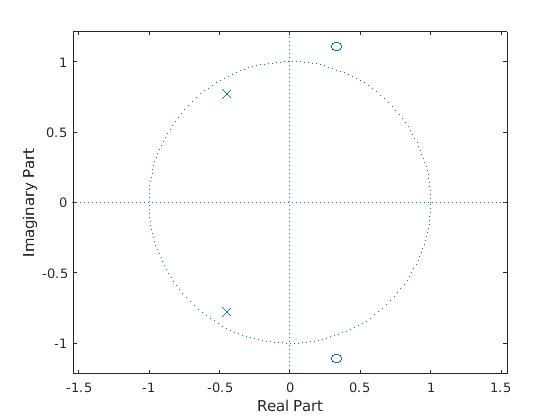
\includegraphics[width=1\textwidth]{./Images/zplane_H}\\
        \caption{Visualisation des pôles et des zéros du filtre $h_k$}
    \end{minipage}
    \hfill%
    \begin{minipage}[c]{.50\linewidth}
        \centering
        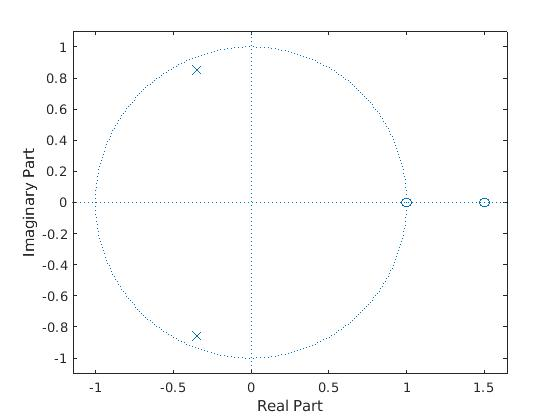
\includegraphics[width=1\textwidth]{./Images/zplane_G}\\
        \caption{Visualisation des pôles et des zéros du filtre $g_k$}
    \end{minipage}
\end{figure}\vspace{0.3cm}

\section{Réponse en fréquence}

Les deux filtres sont réalisables donc leur réponse en fréquence existe :\\


\begin{figure}[H]
    \begin{minipage}[c]{.50\linewidth}
        \centering
        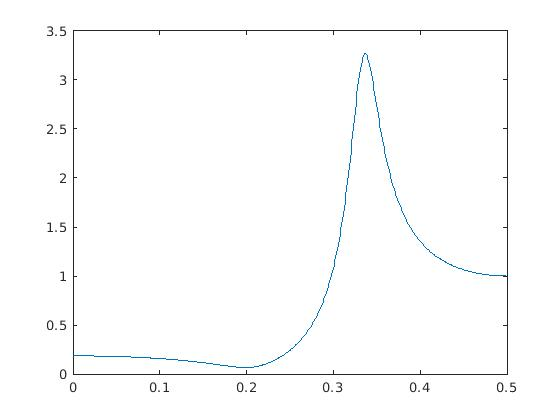
\includegraphics[width=1\textwidth]{./Images/freqz_H}\\
        \caption{Visualisation de $|H(f)|$ sur [0,0.5]}
    \end{minipage}
    \hfill%
    \begin{minipage}[c]{.50\linewidth}
        \centering
        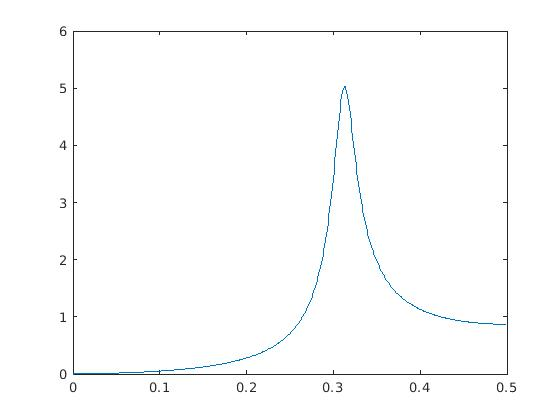
\includegraphics[width=1\textwidth]{./Images/freqz_G}\\
        \caption{Visualisation de $|G(f)|$ sur [0,0.5]}
    \end{minipage}
\end{figure}\vspace{0.3cm}


\chapter{Mise en cascade}

\section{Filtre équivalent}

On met en cascade les filtres $h_k$ et $g_k$. Posons $y_{1k}$ le filtre équivalent à la convolutée tel que : 
$$y_{1k}=h_k*g_k$$

On a :
$$ Y_1(z)=\sum_{k=-\infty}^{\infty}y_{1k}z^{-k}=\sum_{k=-\infty}^{\infty}\left(\sum_{m=-\infty}^{\infty}h_mg_{k-m}\right)z^{-k} $$

On pose $n=k-m$

$$ Y_1(z)=\sum_{n=-\infty}^{\infty}\left(\sum_{m=-\infty}^{\infty}h_mg_n\right)z^{-(n+m)} $$
$$ Y_1(z)=\sum_{n=-\infty}^{\infty}\left(\sum_{m=-\infty}^{\infty}h_mz^{-m}\right)g_nz^{-n} $$

On retrouve
$$ Y_1(z)=H(z)G(z) $$

On sait que \\
$$ Y_1(z)= \frac{(z-z_{1Nh})(z-z_{2Nh})}{(z-z_{1Dh})(z-z_{2Dh})}*\frac{(z-z_{1Ng})(z-z_{2Ng})}{(z-z_{1Dg})(z-z_{2Dg})} $$\\

$\Longrightarrow$ mêmes pôles que $H(z)$ et $G(z)$ donc \textbf{le filtre $y_{1k}$ est réalisable physiquement}.\\

On donc :
$$Y_1(z)= \frac{0.3-0.2z^{-1}+0.4z^{-2}}{1+0.9z^{-1}+0.8z^{-2}}*\frac{0.2-0.5z^{-1}+0.3z^{-2}}{1+0.7z^{-1}+0.85z^{-2}} $$\\

En développant on trouve :
$$Y_1(z)=\frac{0.06-0.19z^{-1}+0.27z^{-2}-0.26z^{-3}+0.12z^{-4}}{1+1.6z^{-1}+2.28z^{-2}+1.325z^{-3}+0.68z^{-4}} $$\\

On peut ainsi représenter les pôles et les zéros de ce filtre sur le plan complexe comme ci-dessous :

\begin{figure}[H]
	\center
	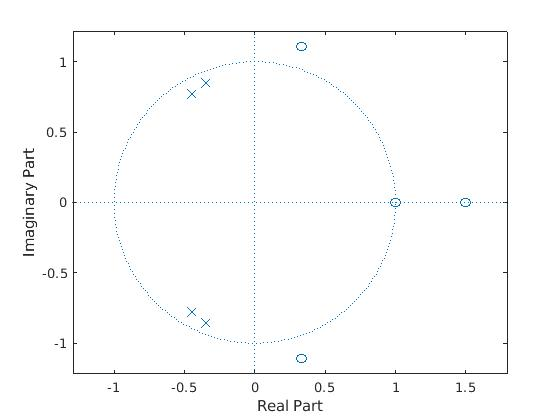
\includegraphics[width=0.7\textwidth]{./Images/zplane_Y1}
	\caption{Visualisation des pôles et des zéros du filtre $y_{1k}$}
\end{figure}\vspace{0.2cm}

On retrouve bien les deux pôles et les deux zéros des filtres respectifs $h_k$ et $g_k$ ce qui est cohérent.\\

On peut également visualiser sa réponse en fréquence ci-dessous :

\begin{figure}[H]
	\center
	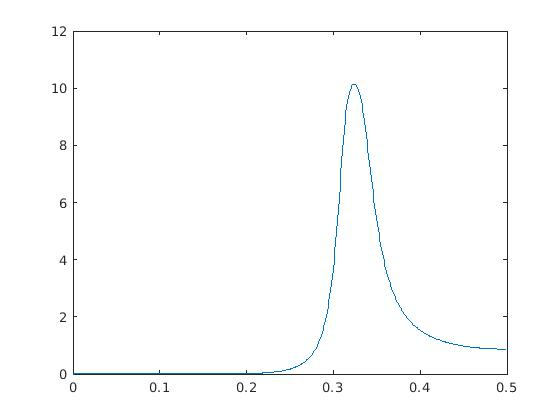
\includegraphics[width=0.7\textwidth]{./Images/freqz_Y1}
	\caption{Visualisation de $|Y_1(f)|$ sur [0,0.5]}
\end{figure}\vspace{0.2cm}


\section{Mise en pratique du filtre}

On crée un signal d'entrée $x_k$ en prenant une fonction sinus sur $[-1;1]$.
À l'aide de la fonction \textbf{filter} sur matlab nous rentrons les données correspondantes au filtre puis nous affichons le signal obtenu en sortie.
\begin{figure}[H]
	\center
	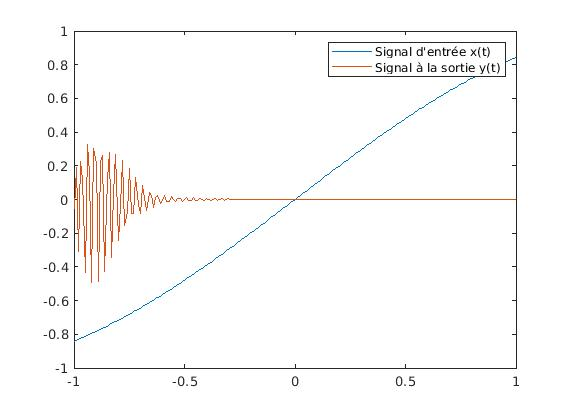
\includegraphics[width=0.7\textwidth]{./Images/filtercascade}
	\caption{Superposition du signal d'entrée et de sortie avec la mise en cascade des deux filtres}
\end{figure}\vspace{0.2cm}

\chapter{Mise en parallèle}

\section{Filtre équivalent}

On met en parallèle les filtres $h_k$ et $g_k$. Posons $y_{2k}$ le filtre équivalent à la convolutée tel que : 
$$y_{2k}=h_k+g_k$$

On a :
$$ Y_2(z)=\sum_{k=-\infty}^{\infty}y_{2k}z^{-k}=\sum_{k=-\infty}^{\infty}(h_k+g_k)z^{-k} $$

D'où :
$$ Y_2(z)=\sum_{k=-\infty}^{\infty}h_kz^{-k}+\sum_{k=-\infty}^{\infty}g_kz^{-k} $$

On retrouve :
$$ Y_2(z)=H(z)+G(z)$$

On sait que :
$$ Y_2(z)= \frac{(z-z_{1Nh})(z-z_{2Nh})}{(z-z_{1Dh})(z-z_{2Dh})}+\frac{(z-z_{1Ng})(z-z_{2Ng})}{(z-z_{1Dg})(z-z_{2Dg})} $$

$$ Y_2(z)= \frac{(z-z_{1Nh})(z-z_{2Nh})(z-z_{1Dg})(z-z_{2Dg})+(z-z_{1Ng})(z-z_{2Ng})(z-z_{1Dh})(z-z_{2Dh})}{(z-z_{1Dh})(z-z_{2Dh})(z-z_{1Dg})(z-z_{2Dg})} $$\\
$\Longrightarrow$ mêmes pôles que $H(z)$ et $G(z)$ donc \textbf{le filtre $y_{2k}$ est réalisable physiquement}.\\


On a donc :\\
$$Y_2(z)=\frac{0.3-0.2z^{-1}+0.4z^{-2}}{1+0.9z^{-1}+0.8z^{-2}}+\frac{0.2-0.5z^{-1}+0.3z^{-2}}{1+0.7z^{-1}+0.85z^{-2}} $$\\

En développant et en sommant on trouve :
$$Y_2(z)=\frac{0.5-0.31z^{-1}+0.525z^{-2}-0.02z^{-3}+0.58z^{-4}}{1+1.6z^{-1}+2.28z^{-2}+1.325z^{-3}+0.68z^{-4}} $$\\

On peut ainsi représenter les pôles et les zéros de ce filtre sur le plan complexe comme ci-dessous :

\begin{figure}[H]
	\center
	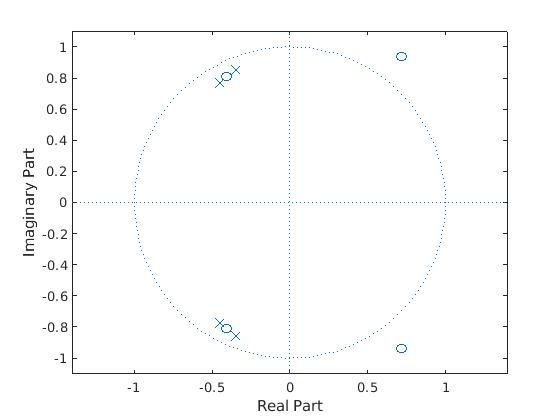
\includegraphics[width=0.7\textwidth]{./Images/zplane_Y2}
	\caption{Visualisation des pôles et des zéros du filtre $y_{2k}$}
\end{figure}\vspace{0.2cm}

On retrouve bien les deux pôles des filtres respectifs $h_k$ et $g_k$. Les zéros de $Y_2(z)$ sont également bien différents de ceux de $H(z)$ et $G(z)$ ce qui est cohérent.\\

On peut également visualiser sa réponse en fréquence ci-dessous :

\begin{figure}[H]
	\center
	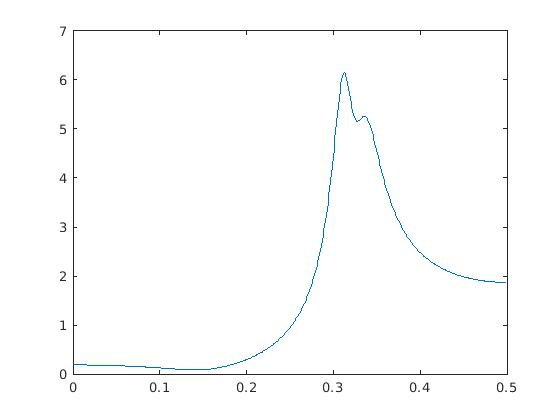
\includegraphics[width=0.7\textwidth]{./Images/freqz_Y2}
	\caption{Visualisation de $|Y_2(f)|$ sur [0,0.5]}
\end{figure}\vspace{0.2cm}


\section{Mise en pratique du filtre}

De même mais cette fois pour la mise en parallèle des deux filtres. On crée un signal d'entrée $x_k$ en prenant une fonction sinus sur $[-1;1]$.
À l'aide de la fonction \textbf{filter} sur matlab nous rentrons les données correspondantes au filtre puis nous affichons le signal obtenu en sortie.

\begin{figure}[H]
	\center
	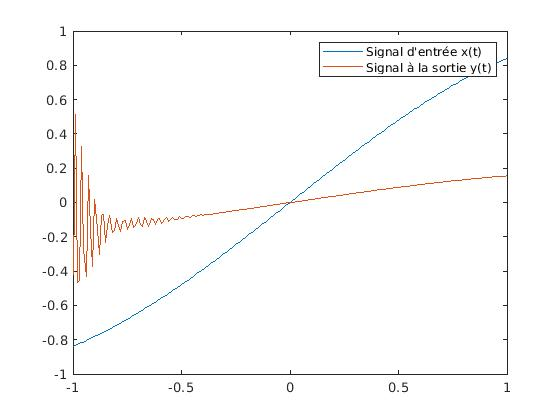
\includegraphics[width=0.7\textwidth]{./Images/filterparallele}
	\caption{Superposition du signal d'entrée et de sortie avec la mise en parallèle des deux filtres}
\end{figure}\vspace{0.2cm}


\chapter*{Conclusion}
\addcontentsline{toc}{chapter}{Conclusion}

Pour conclure, rappelons tout d'abord le sujet de ce projet. Nous avions deux filtres linéaires données par leur transformée en $z$. Nous avons pu tout d'abord analyser si ces mêmes filtres étaient réalisables physiquement d'un point de vue purement mathématique, avec la recherche des valeurs des pôles et zéros de chaque filtre en résolvant une équation du second degré. Nous avons obtenu principalement des valeurs remarquables complexes et il a fallu vérifier si les pôles appartenaient au cercle unité afin d'en conclure la réalisabilité physique des deux filtres. Pour le percevoir de façon concrète nous avons tracé à l'aide du logiciel Matlab les valeurs des pôles et zéros afin de valider nos calculs graphiquement.\\


Dans un second temps nous avons étudié les effets d'une combinaison de ces deux filtres de deux manières différentes.\\
Premièrement en mettant les filtres en cascade/série. Nous avons alors étudié de nouveau la réalisation de ce nouveau filtre ainsi que son effet sur un signal quelconque ,en l'occurrence un simple sinus.\\
Deuxièmement en mettant les filtres en parallèles. Nous nous sommes intéressés de même à la réalisation de ce nouveau filtre puis à son effet sur un signal d'entrée.\\
Dans les deux cas nous avons retracé les pôles et les zéros de nos filtres pour confirmer nos calculs.\\


Ce projet avait donc pour objectif de travailler sur les filtres linéaires et leurs effets sur un signal. Nous avons vu pour deux filtres possédant un effet propre à chacun. L'effet obtenu lors de la combinaison des deux n'étaient pas forcément le même si l'on mettait les filtres en série ou en parallèle. On pourrait donc imaginer la même chose avec plus de filtres.\\

Pour finir ce projet nous aura permis d'accroître nos connaissances sur les filtres linéaires ainsi que nos compétences sur un logiciel tel que Matlab, très utilisé dans le traitement de signal. 


\end{document}
